\documentclass[border=10pt]{standalone}
\usepackage{pgfplots}
\pgfplotsset{compat=1.18}
\begin{document}
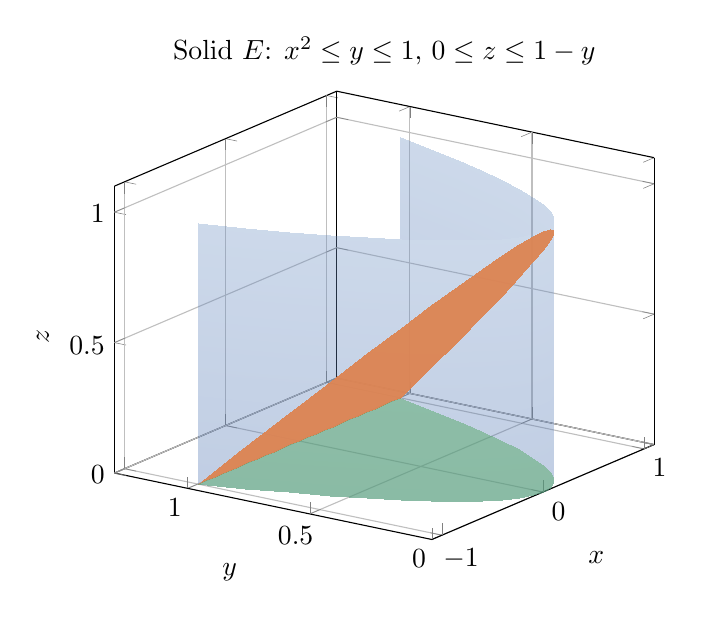
\begin{tikzpicture}
\begin{axis}[
    view={-55}{22},
    xlabel={$x$}, ylabel={$y$}, zlabel={$z$},
    xmin=-1.1, xmax=1.1, ymin=0, ymax=1.3, zmin=0, zmax=1.1,
    title={Solid $E$: $x^2\le y\le 1$, $0\le z\le 1-y$},
    grid, z buffer=sort]
% wall: parabolic cylinder y = x^2 (semi-transparent)
\addplot3[surf, shader=interp, opacity=0.35, draw=black!30,
    colormap={blu}{rgb255=(76,114,176) rgb255=(110,145,195)},
    domain=-1:1, y domain=0:1, samples=25, samples y=12]
    ({x}, {x^2}, {y});
% top: z = 1 - y over shadow D
\addplot3[surf, shader=interp, opacity=0.95, draw=black!30,
    colormap={org}{rgb255=(221,132,82) rgb255=(221,132,82)},
    domain=-1:1, y domain=0:1, samples=25, samples y=15]
    ({x}, {x^2 + y*(1-x^2)}, {1 - x^2 - y*(1-x^2)});
% bottom: z = 0 over shadow D
\addplot3[surf, shader=interp, opacity=0.5, draw=black!30,
    colormap={grn}{rgb255=(85,168,104) rgb255=(85,168,104)},
    domain=-1:1, y domain=0:1, samples=25, samples y=15]
    ({x}, {x^2 + y*(1-x^2)}, {0});
\end{axis}
\end{tikzpicture}
\end{document}